\section{Andamento del pretraining}\label{sec:curve-pretraining-stera30m}

La \autoref{fig:stera30m-pretraining} riporta la perdita sui batch di addestramento, registrata ogni 20 aggiornamenti, la NLL sul campione DEV fisso e il profilo del learning rate.

\begin{figure}[htbp]
\centering
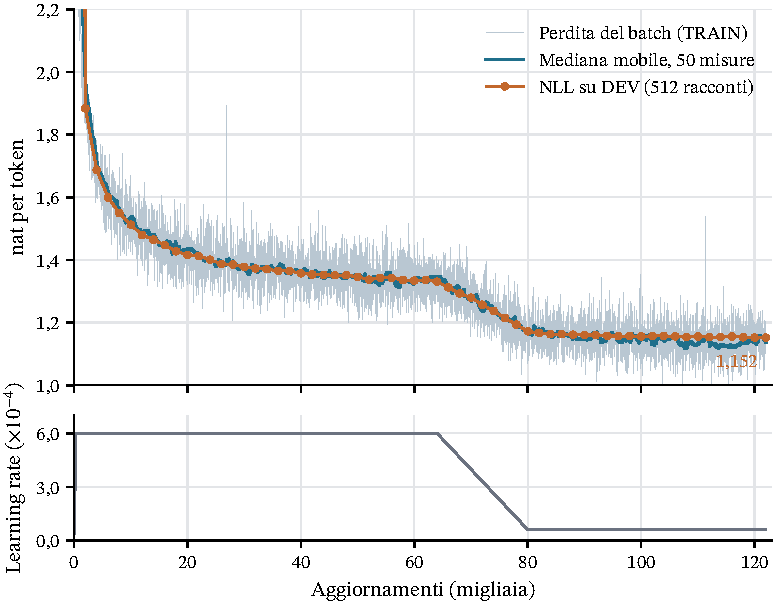
\includegraphics[width=.92\linewidth]{figure/STERA30M/06_pretraining_stera30m.pdf}
\caption{Pretraining di STERA 30M: \num{122000} aggiornamenti e \num{1529514422} token target. In alto, perdita dei batch TRAIN con mediana mobile e NLL sul campione DEV fisso; in basso, learning rate.}
\label{fig:stera30m-pretraining}
\end{figure}

Prima del primo aggiornamento la NLL su DEV è $10{,}928$, prossima a $\ln 50257\approx10{,}82$, il valore di una distribuzione uniforme sul vocabolario. La discesa è rapida nei primi \num{10000} aggiornamenti e prosegue lentamente durante la fase a tasso costante, fino a circa $1{,}33$ al passo \num{64000}. La discesa lineare del learning rate produce un secondo calo marcato, fino a $1{,}172$ al passo \num{80000}. Nella fase finale a tasso ridotto la NLL continua a diminuire lentamente e raggiunge $1{,}152$ (perplessità $3{,}17$) al passo \num{122000}. La perdita su TRAIN e la NLL su DEV restano sovrapposte per tutta la durata dell'addestramento: non si osservano segni di sovradattamento.
